\chapter{Use Cases}

This chapter presents three use cases of interactive slice visualization in the context of biomedical imaging using the slicevis packge. All necessary datasets are included in the repository, as mentioned in the previous chapter. 

\section{Whole-Body Murine CT Scans}
The first use case is a micro CT scan of a laboratory mouse. The image file is called CT280.gff and a corresponding organ segmentation is included as CT280\_organs.segff. Both files were published in an open access manner as part of a paper by Rosenthal et al. [REF].

GFF metadata includes name and color of each class. There is no validation segmentation for this use case.

\begin{figure}[h]
	\centering
	\begin{subfigure}[t]{0.4\linewidth}
		\centering
		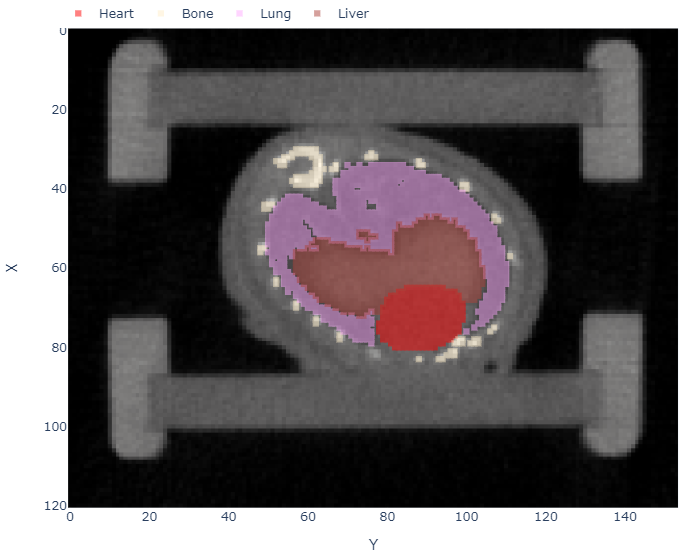
\includegraphics[width=\linewidth]{figures/mouse_axial.png}
		\caption{Axial slice.}
	\end{subfigure}
	\hfill
	\begin{subfigure}[t]{0.55\linewidth}
		\centering
		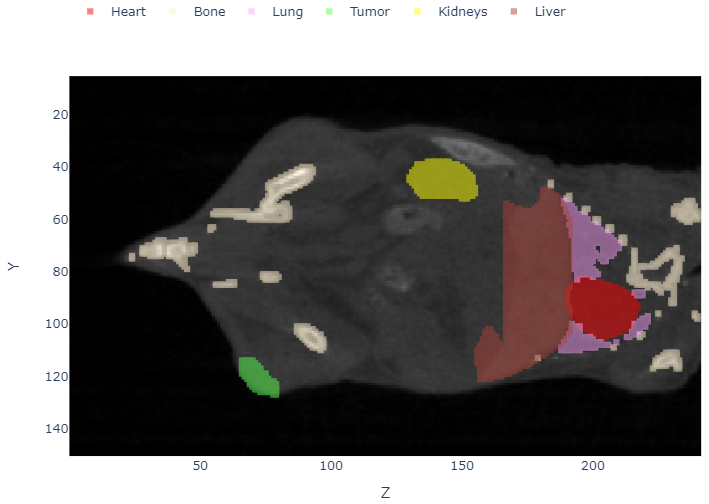
\includegraphics[width=\linewidth]{figures/mouse_coronal.png}
		\caption{Coronal slice.}
	\end{subfigure}
\end{figure}

\section{Lung Tumors}
The second example is a CT scan of a human upper body which was published by The Cancer Imaging Archive. The file is title lung.nii.gz in the examples directory. It is only one of 95 published scans as part of a database to train machine learning models to detect lung cancer. It was republished as part of the Medical Segmentation Decathlon [REF] with a CC-BY-SA license.

The scan is very high resolution and thus large in size, which makes slice visualization computationally more demanding.

Labels of lung nodules, segmented by trained radiologist, are included as lung\_labels.nii.gz. By loading both the image and the labels after each other in SliceWidget, one can precisely locate the tumors, zoom in and visually evaluate the segmentation precision.

\begin{figure}[h]
	\centering
	\begin{subfigure}[t]{0.45\linewidth}
		\centering
		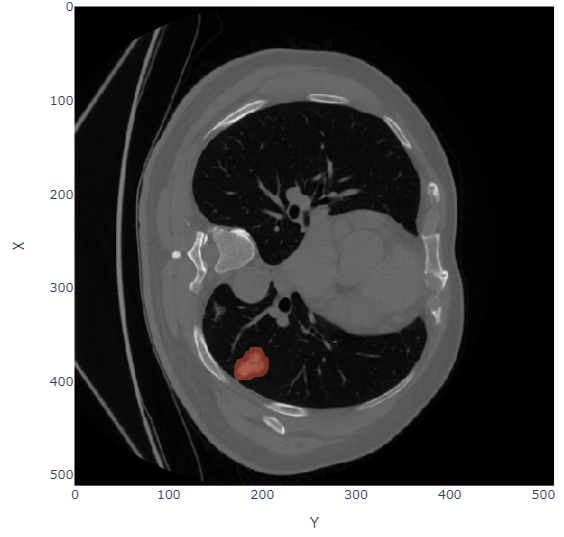
\includegraphics[width=\linewidth]{figures/lung_label.png}
		\caption{Axial slice with labeled tumor.}
	\end{subfigure}
	\hfill
	\begin{subfigure}[t]{0.45\linewidth}
		\centering
		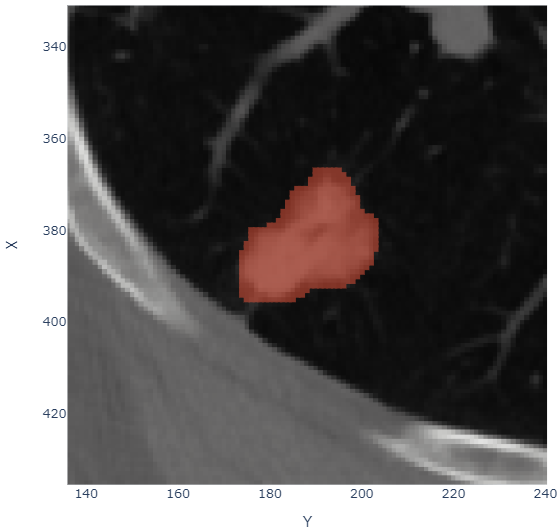
\includegraphics[width=\linewidth]{figures/lung_zoom.png}
		\caption{Zoomed in.}
	\end{subfigure}
\end{figure}

\section{nnU-Net Prediction}
The third example included in the repository is a prediction of lung tumors by a sophisticated convolutional neural network. The model is call nnU-Net and it was the winner of the Decathlon challenge [REF]. It has an accuracy of 69\% for the lung task.

The file is called lung\_prediciton.nii.gz and it was created by downloading pre-trained model weights and executing a prediction on lung.nii.gz.

The aim is to visualize the prediction on top of the label and validate it using the DICE score.

The DICE score is computed as follows:

It is automatically computed once a validation segmentation is loaded and displayed to the user. 

\begin{figure}[h]
	\centering
	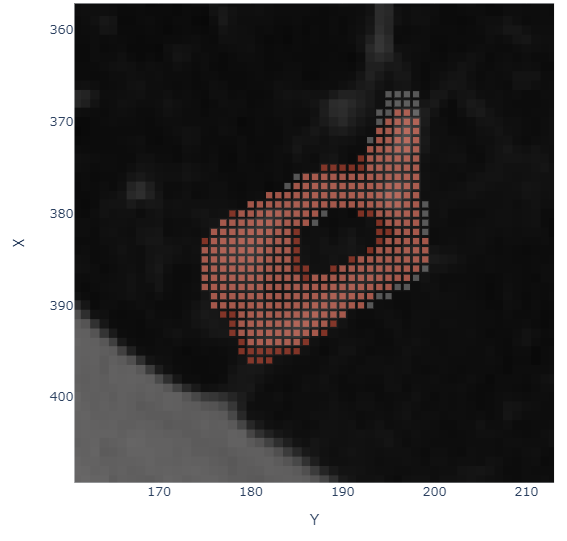
\includegraphics[width=.5\linewidth]{figures/lung_prediction.png}
	\caption{Lung tumor prediction (red) vs. label (white).}
\end{figure}